% Options for packages loaded elsewhere
\PassOptionsToPackage{unicode}{hyperref}
\PassOptionsToPackage{hyphens}{url}
%
\documentclass[
]{book}
\usepackage{amsmath,amssymb}
\usepackage{lmodern}
\usepackage{ifxetex,ifluatex}
\ifnum 0\ifxetex 1\fi\ifluatex 1\fi=0 % if pdftex
  \usepackage[T1]{fontenc}
  \usepackage[utf8]{inputenc}
  \usepackage{textcomp} % provide euro and other symbols
\else % if luatex or xetex
  \usepackage{unicode-math}
  \defaultfontfeatures{Scale=MatchLowercase}
  \defaultfontfeatures[\rmfamily]{Ligatures=TeX,Scale=1}
\fi
% Use upquote if available, for straight quotes in verbatim environments
\IfFileExists{upquote.sty}{\usepackage{upquote}}{}
\IfFileExists{microtype.sty}{% use microtype if available
  \usepackage[]{microtype}
  \UseMicrotypeSet[protrusion]{basicmath} % disable protrusion for tt fonts
}{}
\makeatletter
\@ifundefined{KOMAClassName}{% if non-KOMA class
  \IfFileExists{parskip.sty}{%
    \usepackage{parskip}
  }{% else
    \setlength{\parindent}{0pt}
    \setlength{\parskip}{6pt plus 2pt minus 1pt}}
}{% if KOMA class
  \KOMAoptions{parskip=half}}
\makeatother
\usepackage{xcolor}
\IfFileExists{xurl.sty}{\usepackage{xurl}}{} % add URL line breaks if available
\IfFileExists{bookmark.sty}{\usepackage{bookmark}}{\usepackage{hyperref}}
\hypersetup{
  pdftitle={AMAT- Ciencia de Datos y Machine Learning 2},
  pdfauthor={Karina Lizette Gamboa Puente; Oscar Arturo Bringas López},
  hidelinks,
  pdfcreator={LaTeX via pandoc}}
\urlstyle{same} % disable monospaced font for URLs
\usepackage{longtable,booktabs,array}
\usepackage{calc} % for calculating minipage widths
% Correct order of tables after \paragraph or \subparagraph
\usepackage{etoolbox}
\makeatletter
\patchcmd\longtable{\par}{\if@noskipsec\mbox{}\fi\par}{}{}
\makeatother
% Allow footnotes in longtable head/foot
\IfFileExists{footnotehyper.sty}{\usepackage{footnotehyper}}{\usepackage{footnote}}
\makesavenoteenv{longtable}
\usepackage{graphicx}
\makeatletter
\def\maxwidth{\ifdim\Gin@nat@width>\linewidth\linewidth\else\Gin@nat@width\fi}
\def\maxheight{\ifdim\Gin@nat@height>\textheight\textheight\else\Gin@nat@height\fi}
\makeatother
% Scale images if necessary, so that they will not overflow the page
% margins by default, and it is still possible to overwrite the defaults
% using explicit options in \includegraphics[width, height, ...]{}
\setkeys{Gin}{width=\maxwidth,height=\maxheight,keepaspectratio}
% Set default figure placement to htbp
\makeatletter
\def\fps@figure{htbp}
\makeatother
\setlength{\emergencystretch}{3em} % prevent overfull lines
\providecommand{\tightlist}{%
  \setlength{\itemsep}{0pt}\setlength{\parskip}{0pt}}
\setcounter{secnumdepth}{5}
\usepackage{booktabs}
\ifluatex
  \usepackage{selnolig}  % disable illegal ligatures
\fi
\usepackage[]{natbib}
\bibliographystyle{apalike}

\title{AMAT- Ciencia de Datos y Machine Learning 2}
\author{Karina Lizette Gamboa Puente \and Oscar Arturo Bringas López}
\date{}

\begin{document}
\maketitle

{
\setcounter{tocdepth}{1}
\tableofcontents
}
\hypertarget{bienvenida}{%
\chapter{BIENVENIDA}\label{bienvenida}}

\hypertarget{objetivo}{%
\section{Objetivo}\label{objetivo}}

Desarrollar conocimiento y habilidades para implementar modelos complejos de Machine Learning a través de un flujo de trabajo limpio, ordenado y sistematizado a mediante las librerías en \emph{R} más novedosas que han sido desarrolladas hasta el momento. Al finalizar este curso, el participante será capáz de combinar distintas clases de modelos para dar una solución compleja y precisa a problemas predictivos. Aprenderá a cuantificar los problemas éticos asociados al sesgo o inequidad producidos por modelos de machine learning, así como su interpretación en el mundo productivo. Finalmente, se estudiará la manera de desarrollar un diseño de experimento para implementarse en el ámbito empresarial de modo que el participante pueda tomar mejores decisiones para contribuir en su ambiente laboral.

\textbf{Se asume que el alumno tiene conocimientos generales de estadística, bases matemáticas y de programación básica en R y que cuenta con los conocimientos teóricos básicos de machine learning y prácticos con tidymodels.}

\hypertarget{quienes-somos}{%
\section{¿Quienes somos?}\label{quienes-somos}}

\textbf{ACT. ARTURO BRINGAS}

\textbf{LinkedIn:} \href{https://www.linkedin.com/in/arturo-bringas/}{arturo-bringas}
\textbf{Email:} \href{mailto:act.arturo.b@ciencias.unam.mx}{\nolinkurl{act.arturo.b@ciencias.unam.mx}}

Actuario, egresado de la Facultad de Ciencias y Maestría en Ciencia de Datos, ITAM.
Experiencia en modelos predictivos y de clasificación de machine learning aplicado a seguros, deportes y movilidad internacional. Es jefe de departamento en Investigación Aplicada y Opinión de la UNAM, donde realiza estudios estadísticos de impacto social. Es consultor para empresas y organizaciones como GNP, El Universal, UNAM, Sinnia, la Organización de las Naciones Unidas Contra la Droga y el Delito (UNODC), entre otros. Actualmente es profesor de \emph{ciencia de datos y machine learning} en AMAT y se desempeña como consultor independiente en diferentes proyectos contribuyendo a empresas en temas de machine learning, estadística, series de tiempo, visualización de datos y análisis geoespacial.

\begin{center}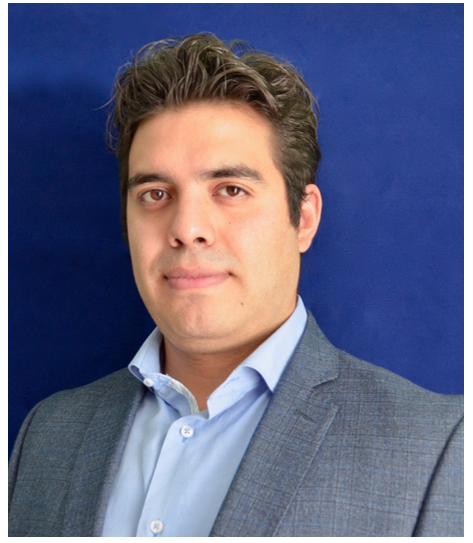
\includegraphics[width=6.57in]{img/00-presentacion/arturo} \end{center}

\textbf{ACT. KARINA LIZETTE GAMBOA}

\textbf{LinkedIn:} \href{https://www.linkedin.com/in/kalizzygam/}{KaLizzyGam}
\textbf{Email:} \href{mailto:lizzygamboa@ciencias.unam.mx}{\nolinkurl{lizzygamboa@ciencias.unam.mx}}

Actuaria, egresada de la Facultad de Ciencias, UNAM, candidata a Maestra en
Ciencia de Datos por el ITAM.

Experiencia en áreas de analítica predictiva e inteligencia del negocio. Lead y Senior
Data Scientist en consultoría en diferentes sectores como tecnología, asegurador,
financiero y bancario. Experta en entendimiento de negocio para la correcta
implementación de algoritmos de inteligencia y explotación de datos.
Actualmente se desarrolla como Arquitecta de Soluciones Analíticas en Merama,
startup mexicana clasificada como uno de los nuevos unicornios de Latinoamérica.
Senior Data Science en CLOSTER y como profesora del diplomado de Metodología
de la Investigación Social por la UNAM así como instructora de cursos de Ciencia de
Datos en AMAT.

Empresas anteriores: GNP, Activer Banco y Casa de Bolsa, PlayCity Casinos,
RakenDataGroup Consulting, entre otros.

\begin{center}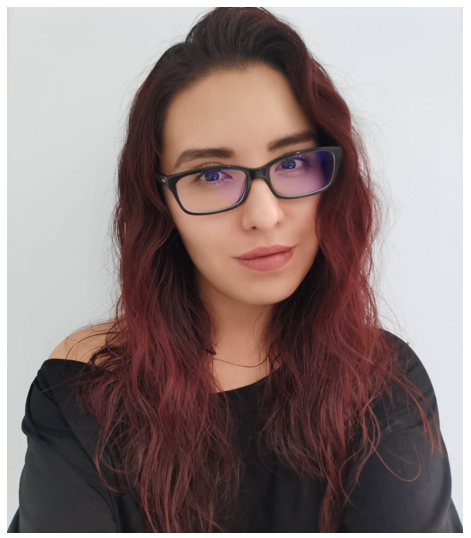
\includegraphics[width=6.54in]{img/00-presentacion/lizzy} \end{center}

\hypertarget{ciencia-de-datos-en-r}{%
\section{Ciencia de Datos en R}\label{ciencia-de-datos-en-r}}

\begin{center}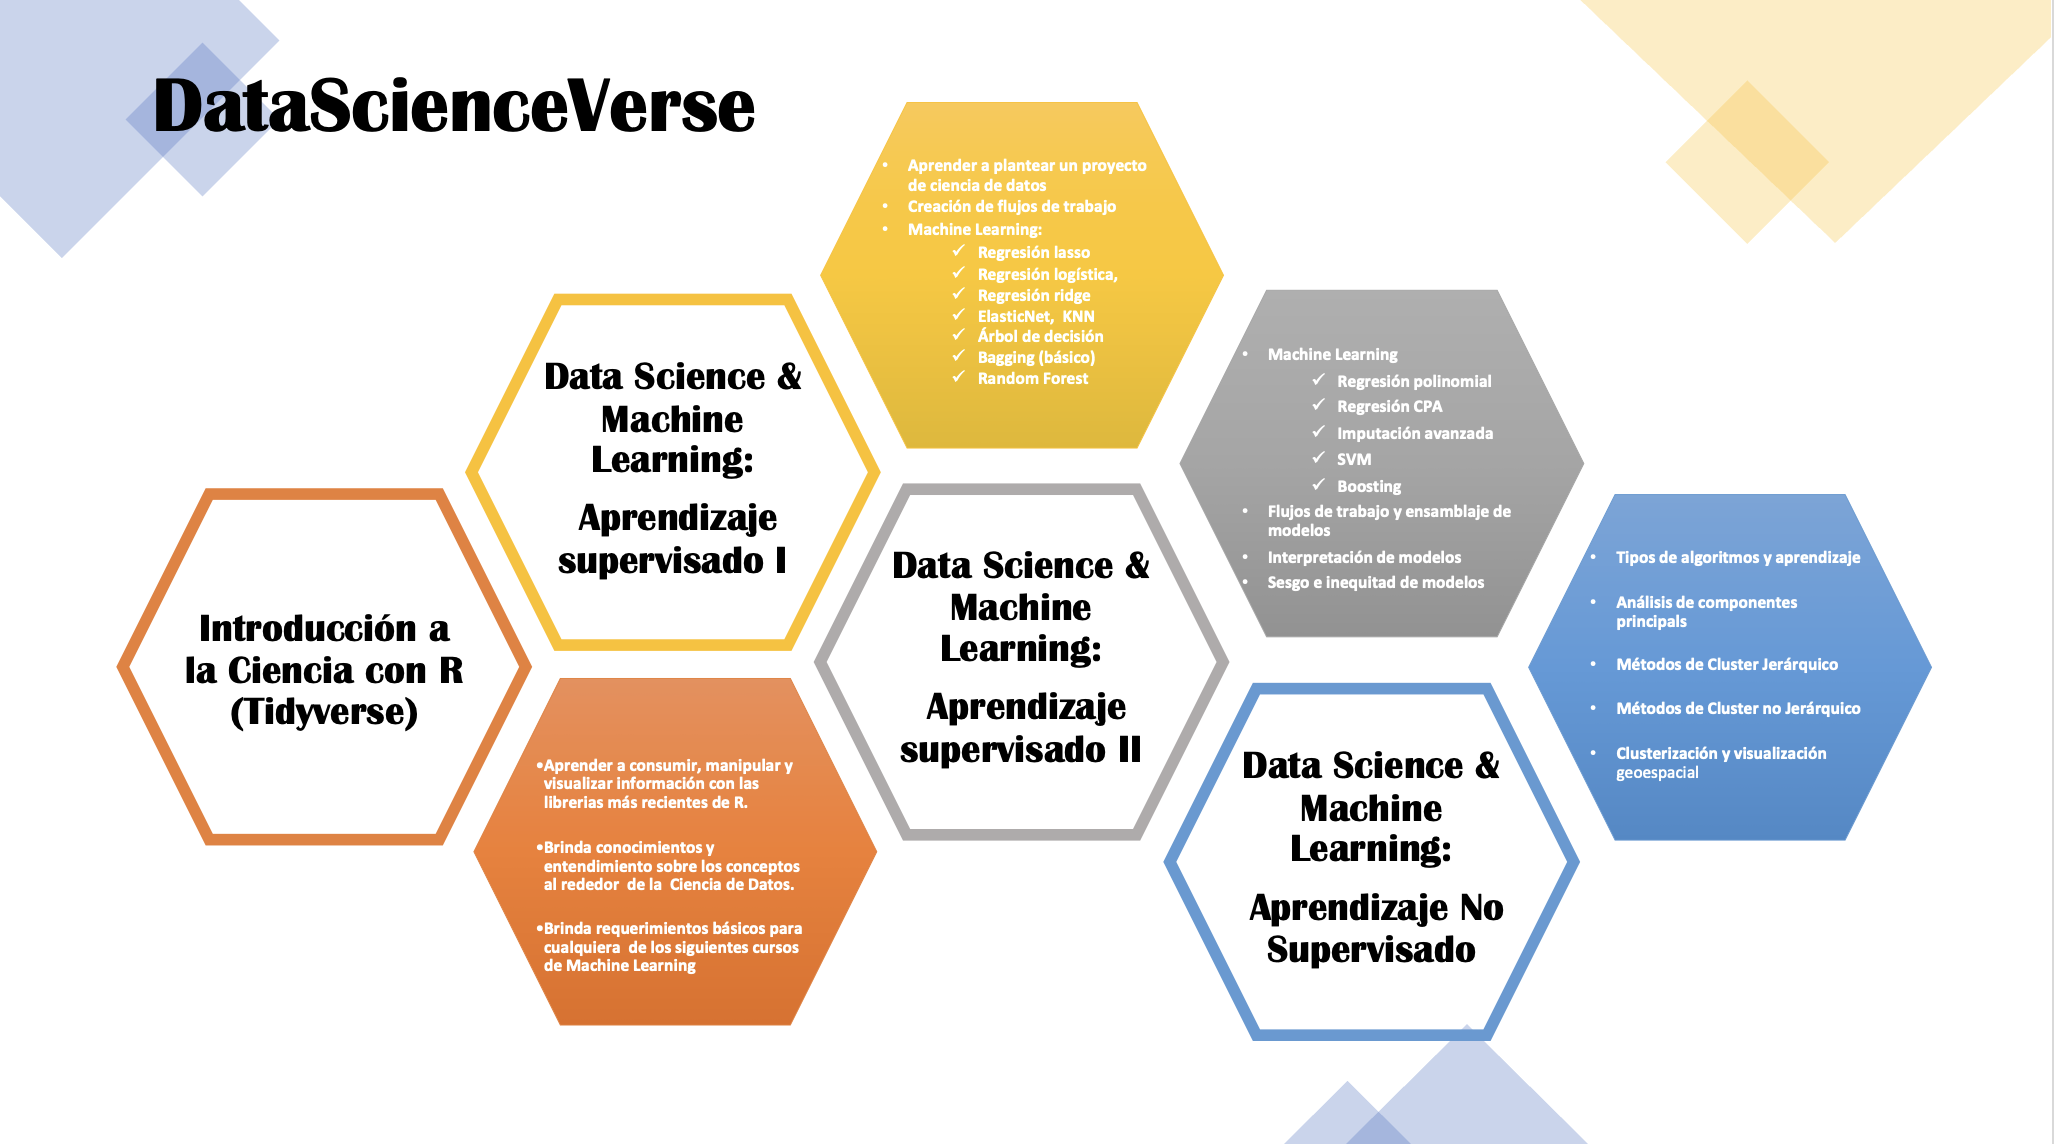
\includegraphics[width=28.53in]{img/00-presentacion/DataScienceVerse} \end{center}

\hypertarget{estructura-del-curso-actual}{%
\section{Estructura del curso actual}\label{estructura-del-curso-actual}}

\hypertarget{alcances-del-curso}{%
\subsection{Alcances del curso}\label{alcances-del-curso}}

Al finalizar el módulo, el participante sabrá plantear un proyecto de ciencia de datos, desde sus requerimientos hasta sus implementación comercial. Sabrá crear flujos de trabajo limpios y ordenados para crear poderosos modelos de Machine Learning. Podrá comparar múltiples modelos y seleccionar el que más aportación realice a su negocio considerando la ética alrededor del sesgo e inequidad producida por modelos. Profundizará su conocimiento en la interpretación de modelos complejos y aprenderá a cuantificar el beneficio comercial de la implementación de modelos.

\textbf{Requisitos:}

\begin{quote}
Computadora con al menos 4Gb Ram.
\end{quote}

\begin{quote}
Instalación de R con al menos versión 4.1.0
\end{quote}

\begin{quote}
Instalación de Rstudio con al menos versión 1.4
\end{quote}

\begin{quote}
Data Science \& Machine Learning (Aprendizaje Supervisado I)
\end{quote}

\textbf{Temario:}

\textbf{1.- Machine Learning (10 HRS)}

\begin{itemize}
\tightlist
\item
  Regresión polinomial
\item
  Regresión con CPA
\item
  Imputación
\item
  SVM
\item
  Boosting
\end{itemize}

\textbf{2. Flujos de trabajo y ensamblajes (8 HRS)}

\begin{itemize}
\tightlist
\item
  Pipelines
\item
  Workflowsets
\item
  Comparación de modelos
\item
  Stacking
\end{itemize}

\textbf{3. Sesgo e inequidad de modelos (4 HRS)}

\begin{itemize}
\tightlist
\item
  Cuantificación de sesgo
\item
  Cuantificación de inequidad
\end{itemize}

\textbf{4. Interpretación de modelos (4 HRS)}

\begin{itemize}
\tightlist
\item
  LIME
\item
  ghv
\end{itemize}

\textbf{5. Aplicación a negocios (6 HRS)}

\begin{itemize}
\tightlist
\item
  Diseño de experimentos en campañas de retención
\item
  Valuación de implementación de modelos
\end{itemize}

\hypertarget{duraciuxf3n-y-evaluaciuxf3n-del-curso}{%
\section{Duración y evaluación del curso}\label{duraciuxf3n-y-evaluaciuxf3n-del-curso}}

\begin{itemize}
\item
  El programa tiene una duración de 32 hrs.
\item
  Las clases serán impartidas los días domingo, de 9:00 am a 1:00 pm
\item
  Serán asignados ejercicios que el participante deberá resolver entre una semana y otra.
\item
  Al final del curso se solicitará un proyecto final, el cual \textbf{deberá ser entregado para ser acreedor a la constancia de participación}.
\end{itemize}

\hypertarget{recursos-y-dinuxe1mica-de-clase}{%
\section{Recursos y dinámica de clase}\label{recursos-y-dinuxe1mica-de-clase}}

En esta clase estaremos usando:

\begin{itemize}
\tightlist
\item
  R \href{https://cran.r-project.org/}{da click aquí si aún no lo descargas}
\item
  RStudio \href{https://www.rstudio.com/products/rstudio/download/}{da click aquí también}
\item
  Miro \href{https://miro.com/welcomeonboard/c3huendzNURhRUVGbHlsWGVFYlBBMXRaSncybXRrbjBRU2R5WWg2eDFKUXY1VlJ1SGJFdmc4ZmRuWEgwcllpenwzMDc0NDU3MzYxMzQwNDIyODEy?invite_link_id=152058640259}{úsame}
\item
  Zoom \href{https://us02web.zoom.us/j/5155440751?pwd=YzJCOGF0VnlZdlZlS0Fpc3MvZEhadz09}{Clases}

  \begin{itemize}
  \tightlist
  \item
    Pulgar arriba: Voy bien, estoy entendiendo!
  \item
    Pulgar abajo: Eso no quedó muy claro
  \item
    Mano arriba: Quiero participar/preguntar ó Ya estoy listo para iniciar
  \end{itemize}
\item
  Grupo de WhatsApp \href{https://chat.whatsapp.com/KUbqIk8Cqu42zkXffIgUQQ}{El chismecito está aquí}
\item
  \href{https://drive.google.com/drive/folders/1IblKYfDpSjV89FBT3c-PafOiD4wW7UrD?usp=sharing}{Google Drive}
\item
  Notas de clase \href{KaLizzyGam.github.io/index.html}{Revisame si quieres aprender}
\item
  Documento del taller de \href{https://docs.google.com/spreadsheets/d/1hCRt00nYyZvbkfi9yOMRSR0R30lPRtKzaNKKlgAE78M/edit?usp=sharing}{Scoping}.
\end{itemize}

\hypertarget{intro}{%
\chapter{Introduction}\label{intro}}

  \bibliography{book.bib,packages.bib}

\end{document}
